%!TEX program = xelatex
%!TEX root = ../all_short.tex

\chapter{Linear classification: A Summary}

\section*{Introduction to Classification}

\begin{itemize}
    \item Classification predicts discrete outcomes (class labels) rather than continuous values.
    \item Input space partitioned into \alert{decision regions}, each corresponding to a class.
    \item \alert{Linear classification models}: decision boundaries are hyperplanes in feature space.
    \item Datasets separable by such boundaries are \alert{linearly separable}.
    \item Target representation:
    \begin{itemize}
        \item Binary: $t\in\{0,1\}$.
        \item Multiclass ($K>2$): \alert{1-of-$K$ coding} (vector of $K$ bits, exactly one 1).
    \end{itemize}
\end{itemize}

\subsection*{Three Approaches to Classification}

\begin{enumerate}
    \item \alert{Discriminant function}: direct mapping $f:\X\mapsto\{1,\ldots,K\}$.
    \item \alert{Discriminative approach}: infer $p(C_{j}|\x)$ (inference), then assign class (decision).
    \item \alert{Generative approach}: model $p(\x|C_{j})$ and $p(C_{j})$, derive posteriors via Bayes.
\end{enumerate}

\begin{itemize}
    \item Approaches 1 and 2 are \alert{discriminative} (directly tackle classification).
    \item For classification, adapt linear regression via \alert{generalized linear model}:
    \begin{myequation}
    h(\x;\w,b)=f(\w^T\x+b)
    \end{myequation}
    with $f$ an \alert{activation function} mapping to $[0,1]$.
    \item Decision boundaries: $\w^T\x+b=f^{-1}(c)$ (linear in feature space). $f^{-1}$ is \alert{link function}.
    \item Generative approach: define probabilistic models for items within each class based on training data.
\end{itemize}

\section*{Binary Classification with Linear Discriminants}

\begin{itemize}
    \item Equation $\w^T\x + b = 0$ defines a hyperplane in $\mathbb{R}^d$.
    \item For $\x_0$ on hyperplane: $\w^T\x_0 + b = 0 \implies b = -\w^T\x_0$, giving $\w^T(\x - \x_0) = 0$.
    \item $\w$ is a normal vector (perpendicular to every vector lying in the hyperplane).
    \item $\w^T\x$ measures alignment with $\w$; hyperplane is level set of this linear functional.
    \item Normalized form: $\frac{\w^T}{\|\w\|}\x + \frac{b}{\|\w\|} = 0$, where $\frac{\w}{\|\w\|}$ is unit normal.
    \item $\frac{|b|}{\|\w\|}$ is perpendicular distance from origin to hyperplane.
    \item Sign of $\w^T\x + b$ indicates which side: positive $\Rightarrow$ side $\w$ points to, negative $\Rightarrow$ opposite.
    \item Magnitude $|\w^T\x + b|$ measures distance from decision boundary.
    \item Bias $b$ shifts hyperplane along direction of $\w$.
    \item For classification with $t\in\{-1,+1\}$: correct classification when $t(\w^T\x + b) > 0$ (point on correct side with margin).
    \item Magnitude $|t(\w^T\x + b)|$ measures classification confidence.
\end{itemize}

\begin{figure}[ht]
\begin{center}
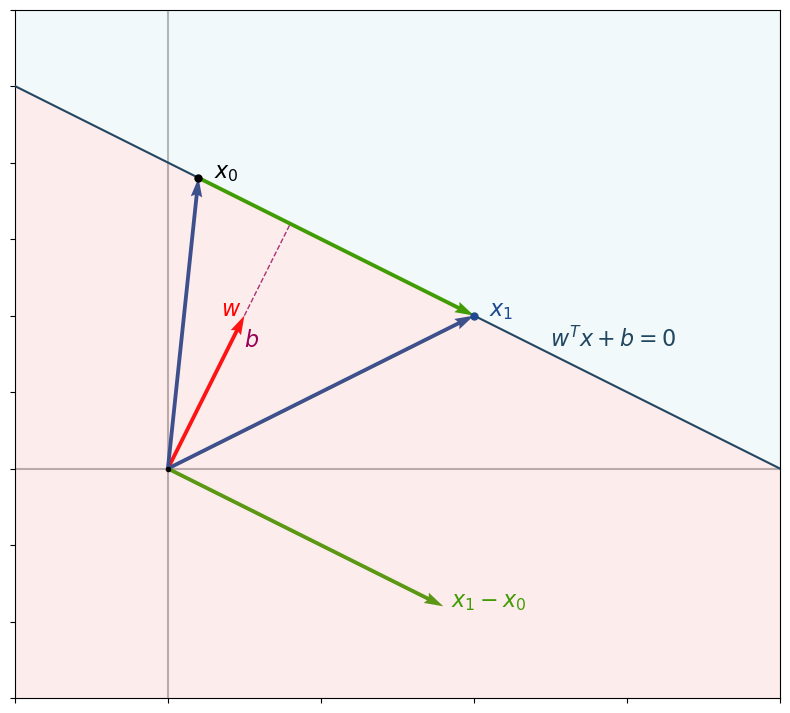
\includegraphics[width=8cm]{figures/hyperplane.png}
\caption{Vector view of hyperplane equation.}
\end{center}
\end{figure}

\begin{figure}[ht]
\begin{center}
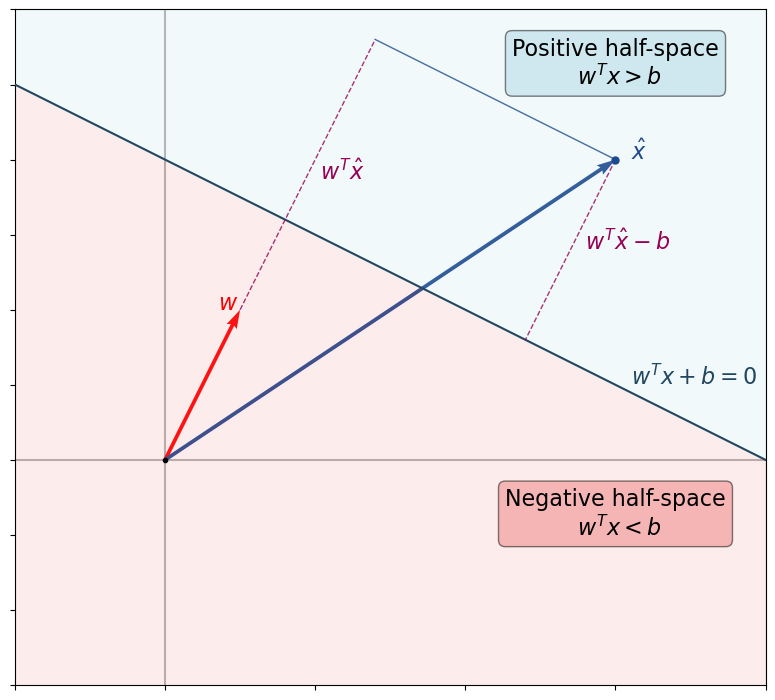
\includegraphics[width=8cm]{figures/hyperplane1.png}
\caption{Positive and negative hyperspaces.}
\end{center}
\end{figure}

\begin{figure}[ht]
\begin{center}
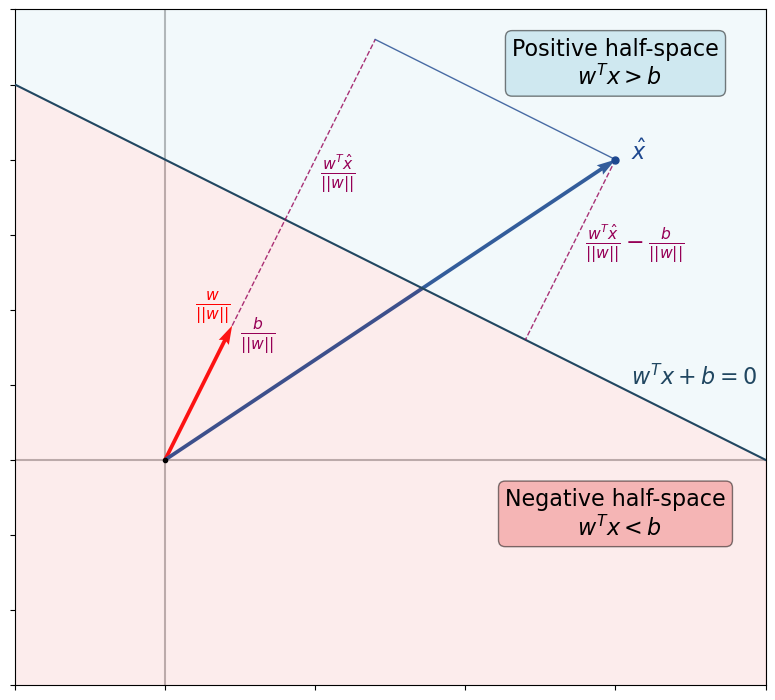
\includegraphics[width=8cm]{figures/hyperplane2.png}
\caption{Normalized distances.}
\end{center}
\end{figure}

\subsection*{Multiclass Extension}

\subsubsection*{One-Versus-Rest}
\begin{itemize}
    \item Train $K-1$ binary classifiers $f_i$, each separating $C_i$ from all other classes.
    \item Decision: if $f_i(\x) > 0$, assign to $C_i$; else continue.
    \item \textbf{Limitation}: Regions may overlap (multiple classifiers positive) or leave gaps (all classifiers negative).
\end{itemize}

\subsubsection*{One-Versus-One}
\begin{itemize}
    \item Train $K(K-1)/2$ classifiers $f_{ij}$ for each pair $(C_i, C_j)$.
    \item Decision by majority voting: each classifier votes for one class.
    \item \textbf{Limitations}: Regions may remain unassigned (ties), $O(K^2)$ complexity, possibility of voting cycles.
\end{itemize}

\subsubsection*{Multiclass Discriminant (Argmax)}
\begin{itemize}
    \item Define $K$ linear functions $y_i(\x) = \w_i^T \x + b_i$.
    \item Classification rule: $k = \arg\max{j}{y_j(\x)}$ (winner-take-all).
    \item Decision boundary between $C_i$ and $C_j$: $y_i(\x) = y_j(\x) \implies (\w_i - \w_j)^T \x + (b_i - b_j) = 0$ (hyperplane).
    \item This partition is complete and unambiguous.
    \item Decision regions are \textbf{convex and connected}. Proof: if $\x_A,\x_B \in \mathcal{R}_k$, then for any convex combination $\hat{\x} = \lambda\x_A + (1-\lambda)\x_B$, $y_k(\hat{\x}) = \lambda y_k(\x_A) + (1-\lambda)y_k(\x_B) > \lambda y_j(\x_A) + (1-\lambda)y_j(\x_B) = y_j(\hat{\x})$ for all $j\neq k$.
    \item Convexity ensures stability under small perturbations.
    \item Trade-off: unified framework requires learning all $K$ weight vectors jointly.
\end{itemize}

\subsubsection*{Beyond Linearity: Quadratic Discriminants}
\begin{itemize}
    \item Incorporate pairwise feature interactions:
    \begin{myequation}
    h(\x;\w,b)=b+\sum_{i=1}^{d}w_{i}x_i+\sum_{i=1}^{d}\sum_{j=1}^{i}w_{ij}x_ix_j
    \end{myequation}
    \item Adds $\frac{d(d+1)}{2}$ new parameters, enabling curved decision boundaries.
    \item Can be seen as linear classifier in expanded feature space (original features + pairwise products).
\end{itemize}

\section*{Least Squares Applied to Classification}

\begin{itemize}
    \item Use 1-of-$K$ coding: $z_{1},\ldots,z_{K}$ with $z_i=1$ for class $C_i$.
    \item Derive $K$ linear regression functions $h_{i}(\x)=\w_i^T\x+b_i$ with $z_i$ as targets.
    \item Classification: assign $\x$ to class $C_k$ where $k=\argmax{i}{h_{i}(\x)}$.
    \item $h_i(\x)$ estimates $\me{z_i|\x}$, which under Bernoulli assumption equals $P(C_i|\x)$ (but not constrained to $[0,1]$).
    \item Training set $(\X,\t)$ with $\x_i\in\Real^{d}$, $\t_i\in\{0,1\}^{K}$.
    \item Predictions: $\y_i=\mathbf{h}(\x_i)=\W\x_i+\mathbf{b}$.
    \item Augmented parameter matrix $\overline{\W}$ (including biases) and design matrix $\overline\X$:
    \begin{myequation}
    \overline{\W}=
     \left(
         \begin{array}{ccccc}
              w_{10} & w_{11} &  \cdots & w_{1d} \\
              w_{20} & w_{21}  &  \cdots & w_{2d} \\
             \vdots & \vdots & \ddots & \vdots \\
              w_{K0} & w_{K1} &  \cdots & w_{Kd}  
         \end{array}
         \right),\quad
    \overline\X=
     \left(
         \begin{array}{cccc}
              1 & x_{11}  &  \cdots & x_{1d} \\
              1 & x_{21}  &  \cdots & x_{2d} \\
              \vdots &  \vdots & \ddots & \vdots \\
              1 & x_{n1}  &  \cdots & x_{nd}  
         \end{array}
         \right)
    \end{myequation}
    \item Predictions matrix: $\overline\Y = \overline\W\overline\X^T$.
    \item Target matrix $\Vbold{T}$ ($K\times n$) with $\Vbold{T}_{ij}=t_{ji}$.
    \item Residual matrix $\Vbold{R}= \overline\W\overline\X^T-\Vbold{T}$.
    \item Sum of squared residuals = $\text{tr}(\Vbold{R}^{T}\Vbold{R})$.
    \item Objective: $E({\overline\W})=\frac{1}{2}\text{tr}(\Vbold{R}^{T}\Vbold{R})$.
    \item Gradient: $\nabla_{\W} E(\overline\W)={\overline \X}^{T}{\overline \X}{\overline\W}-{\overline \X}^{T}\Vbold{T}$.
    \item Closed-form solution:
    \begin{myequation}
    {\overline\W}=({\overline \X}^{T}{\overline \X})^{-1}{\overline \X}^{T}\Vbold{T}
    \end{myequation}
    \item Discriminant functions:
    \begin{myequation}
    \mathbf{h}(\x)={\overline\W}^{T}{\overline \x}=\Vbold{T}^{T}{\overline\X}({\overline\X}^{T}{\overline\X})^{-1}{\overline\x}
    \end{myequation}
    \item \textbf{Limitations}: Predictions not constrained to $[0,1]$, sensitive to outliers and class imbalance.
\end{itemize}

\section*{Fisher Linear Discriminant: Maximizing Class Separability}

\begin{itemize}
    \item Projects data onto lower-dimensional subspace to maximize class separation.
    \item Binary case: project onto direction $\w$: $y=\w^{T}\x$ (assume $\|\w\|=1$).
    \item Classification: choose threshold $\tilde y$, assign $\x$ to $C_1$ if $y>\tilde y$.
\end{itemize}

\subsection*{Deriving Optimal Projection for Binary Classification}

\begin{itemize}
    \item Class means: $\mathbf{m}_{1}=\frac{1}{n_{1}}\sum_{\x\in C_{1}}\x$, $\mathbf{m}_{2}=\frac{1}{n_{2}}\sum_{\x\in C_{2}}\x$.
    \item Projected means: $m_i = \w^T\mathbf{m}_i$.
    \item Maximizing $m_2-m_1$ alone gives $\w = \frac{\mathbf{m}_2-\mathbf{m}_1}{\|\mathbf{m}_2-\mathbf{m}_1\|}$.
    \item \textbf{Limitation}: ignores within-class spread; classes may overlap in projection.
    \item Within-class variance for class $i$: $s_{i}^{2}=\sum_{\x\in C_{i}}(\w^{T}\x-m_{i})^{2}$.
    \item Fisher criterion:
    \begin{myequation}
    J(\w)=\frac{(m_{2}-m_{1})^{2}}{s_{1}^{2}+s_{2}^{2}}
    \end{myequation}
    Maximizes separation while minimizing dispersion.
    \item Within-class covariance matrix: $\S_{i}=\sum_{\x\in C_{i}}(\x-\mathbf{m}_{i})(\x-\mathbf{m}_{i})^{T}$.
    \item Projected variance: $s_i^2 = \w^T\S_i\w$.
    \item Total within-class covariance: $\S_W=\S_1+\S_2$.
    \item Between-class covariance: $\S_{B}=(\mathbf{m}_{2}-\mathbf{m}_{1})(\mathbf{m}_{2}-\mathbf{m}_{1})^{T}$.
    \item Fisher criterion in matrix form:
    \begin{myequation}
    J(\w)=\frac{\w^{T}\S_{B}\w}{\w^{T}\S_{W}\w}
    \end{myequation}
    \item Maximization leads to generalized eigenvalue problem:
    \begin{myequation}
    \S_B\w = \lambda \S_W\w
    \end{myequation}
    \item Solution:
    \begin{myequation}
    \hat\w=\S_W^{-1}(\mathbf{m}_2-\mathbf{m}_1)
    \end{myequation}
    \item $\S_W^{-1}$ acts as whitening transform, down-weighting directions of high variance.
\end{itemize}

\subsection*{Determining the Optimal Threshold}
\begin{itemize}
    \item Assume projected values for each class are Gaussian.
    \item Estimate $m_i$, $\sigma_i^2$ via MLE.
    \item Bayes posterior: $p(C_i|y)\propto p(y|C_i)p(C_i)\propto n_i e^{-\frac{(y-m_i)^2}{2\sigma_i^2}}$.
    \item Optimal threshold where $p(C_1|y)=p(C_2|y)$.
\end{itemize}

\subsection*{Extending LDA to Multiclass Classification}

\begin{itemize}
    \item For $K>2$, find $D'$ projection directions ($1<D'<D$): $y_k=\w_k^T\x$.
    \item Projection matrix $\W$ ($D\times D'$) gives $\y=\W^T\x$.
    \item Within-class scatter:
    \begin{myequation}
    \S_W=\sum_{i=1}^{K}\sum_{\x\in C_{i}}(\x-\mathbf{m}_{i})(\x-\mathbf{m}_{i})^{T}
    \end{myequation}
    \item Total covariance:
    \begin{myequation}
    \S_{T}=\sum_{\x}(\x-\mathbf{m})(\x-\mathbf{m})^{T}=\S_W+\sum_{i=1}^{K}n_{i}(\mathbf{m}_{i}-\mathbf{m})(\mathbf{m}_{i}-\mathbf{m})^{T}
    \end{myequation}
    \item Between-class scatter:
    \begin{myequation}
    \S_B=\sum_{i=1}^{K}n_{i}(\mathbf{m}_{i}-\mathbf{m})(\mathbf{m}_{i}-\mathbf{m})^{T}
    \end{myequation}
    \item Projected scatters: $\mathbf{s}_W=\W^{T}\S_W\W$, $\mathbf{s}_B=\W^{T}\S_B\W$.
    \item Objective functions:
    \begin{itemize}
        \item Determinant ratio: $J_1(\W)=\frac{|\mathbf{s}_B|}{|\mathbf{s}_W|}=|(\W^{T}\S_W\W)^{-1}\W^{T}\S_B\W|$.
        \item Trace ratio: $J_2(\W)=\text{tr}(\mathbf{s}_W^{-1}\mathbf{s}_B)=\text{tr}{(\W^{T}\S_W\W)^{-1}\W^{T}\S_B\W}$.
    \end{itemize}
    \item Solutions via generalized eigenvalue problem: $\S_B\w_i=\lambda_i\S_W\w_i$.
    \item $\W^*$ consists of eigenvectors corresponding to $D'$ largest eigenvalues.
    \item Rank of $\S_B$ at most $\min(K-1, D)$, so maximum meaningful $D' = K-1$.
    \item Steps:
    \begin{enumerate}
        \item Compute $\S_W$, $\S_B$.
        \item Solve $\S_B\w=\lambda\S_W\w$.
        \item Select top $K-1$ eigenvectors.
        \item Form $\W$ and project data.
    \end{enumerate}
    \item \textbf{Limitations}:
    \begin{itemize}
        \item $\S_W$ singular if $n < D$ (need regularization or PCA preprocessing).
        \item Assumes Gaussian classes with equal covariance.
        \item Linear boundaries only.
        \item Sensitive to class imbalance (weighting by $n_i$).
    \end{itemize}
    \item Useful for visualization: project onto first 2 or 3 discriminant directions.
\end{itemize}

\section*{Perceptron}

\begin{itemize}
    \item Foundational neural network model (1960s).
    \item Binary classifier with linear decision boundary:
    \begin{myequation}
    h(\x)=f(\w^T\x+b)=f(\ow^T\ox),\quad f(i)=\begin{cases}
    -1 & i< 0\\
    1 & i\geq 0
    \end{cases}
    \end{myequation}
    \item Targets $t_i\in\{-1,1\}$.
    \item Can only classify linearly separable data.
    \item Cost function based on misclassified points:
    \begin{myequation}
    E_{p}(\ow)=-\sum_{\x_{i}\in{\cal M}}\ow^T\ox_i t_i
    \end{myequation}
    where $\cal M$ is set of misclassified points.
    \item Gradient: $\nabla_{\ow} E_{p}(\ow)=-\sum_{\x_{i}\in{\cal M}}\ox_i t_i$.
    \item Batch gradient descent:
    \begin{myequation}
    \ow^{(k+1)}=\ow^{(k)}+\eta\sum_{\x_{i}\in{\cal M}_{k}}\ox_i t_i
    \end{myequation}
    \item Online (stochastic) version:
    \begin{myequation}
    \ow^{(k+1)}=\ow^{(k)}+\eta\ox_{i}t_i
    \end{myequation}
    for a single misclassified $\x_i$.
    \item For a misclassified point, its cost decreases after update:
    \begin{myalign}
    -\x_{i}^T\w^{(k+1)}t_i &= -\x_{i}^T\w^{(k)}t_i-\eta(\x_{i}t_i)^{T}\x_{i}t_i \\
    &= -\x_{i}^T\w^{(k)}t_i-\eta\|\x_i\|^2 < -\x_{i}^T\w^{(k)}t_i
    \end{myalign}
    \item Correcting one point may cause another to become misclassified, but algorithm guaranteed to converge if data is linearly separable.
\end{itemize}

\subsection*{Convergence of the Perceptron Algorithm}

\begin{itemize}
    \item \textbf{Assumption}: Data linearly separable: $\exists \ow^*$ with $\|\ow^*\|=1$ and $\ow^{*T}\ox_i t_i > 0$ for all $i$.
    \item \textbf{Margin}: $\gamma = \min_i \ow^{*T}\ox_i t_i > 0$.
    \item \textbf{Radius}: $R = \max_i \|\ox_i\|$.
    \item Consider $\ow^{(0)} = \mathbf{0}$ and updates on misclassified points.
\end{itemize}

\subsubsection*{Growth of Alignment with Optimal Separator}
\begin{itemize}
    \item For a misclassified point $\ox_{k+1}, t_{k+1}$:
    \begin{myalign}
    \ow^{(k+1)T}\ow^* &= \ow^{(k)T}\ow^* + \eta\, \ox_{k+1}^T \ow^* t_{k+1} \\
    &\ge \ow^{(k)T}\ow^* + \eta \gamma
    \end{myalign}
    \item After $T$ updates: $\ow^{(T)T}\ow^* \ge T\eta\gamma$.
\end{itemize}

\subsubsection*{Controlled Growth of Weight Vector Norm}
\begin{itemize}
    \item Squared norm update:
    \begin{myalign}
    \|\ow^{(k+1)}\|^2 &= \|\ow^{(k)}\|^2 + 2\eta\, \ow^{(k)T}\ox_{k+1} t_{k+1} + \eta^2 \|\ox_{k+1}\|^2 \\
    &\le \|\ow^{(k)}\|^2 + \eta^2 R^2 \quad (\text{since } \ow^{(k)T}\ox_{k+1} t_{k+1} < 0)
    \end{myalign}
    \item After $k$ updates: $\|\ow^{(k)}\|^2 \le k\eta^2 R^2$, so $\|\ow^{(k)}\| \le \sqrt{k}\eta R$.
\end{itemize}

\subsubsection*{Combining Bounds}
\begin{itemize}
    \item Cauchy-Schwarz: $\ow^{(k)T}\ow^* \le \|\ow^{(k)}\|\,\|\ow^*\| = \|\ow^{(k)}\|$.
    \item Substituting bounds: $k\eta\gamma \le \|\ow^{(k)}\| \le \sqrt{k}\eta R$.
    \item Squaring: $k^2 \eta^2 \gamma^2 \le k \eta^2 R^2$.
    \item Dividing by $k\eta^2$ (for $k>0$):
    \begin{myequation}
    k \le \left(\frac{R}{\gamma}\right)^2
    \end{myequation}
    \item Number of updates bounded by $(R/\gamma)^2$.
    \item Bound independent of dimensionality and dataset size.
    \item Larger margin $\gamma$ $\Rightarrow$ faster convergence.
    \item If data not linearly separable, algorithm may not converge (oscillates).
\end{itemize}

\subsection*{Summary}
\begin{itemize}
    \item Perceptron is simple linear classifier with hard threshold.
    \item Learning by updating weights on misclassified points.
    \item Guaranteed finite-time convergence for linearly separable data.
    \item Convergence bound depends only on margin and data radius.
    \item Limitation: requires linear separability; motivates margin-based methods (SVMs) and nonlinear extensions (neural networks).
\end{itemize}

